\section{FT Prototypes}

Two prototypes of the FT-Cal, with 9 and 16 channels, respectively, were designed, assembled, and tested with
cosmic rays and electron beams to optimize and validate the detector design. Specifically, the prototypes were
used to check the single crystal mechanical assembly, the thermal performance, the front-end and read-out
electronics, and the electrical connections via a motherboard. The response to cosmic rays was studied for both
prototypes, while the response to electromagnetic showers was studied at Jefferson Lab (JLab) and the INFN
Laboratory Nazionali di Frascati (LNF) in Italy. The 9-channel prototype (Proto-9) was tested at JLab using 2-3~GeV
electrons deflected by the Hall~B tagger system~\cite{beamline},  while the 16-channel prototype (Proto-16) was
tested at the Beam Test Facility of LNF with a 0.5~GeV electron beam. Extensive simulations were performed
and compared to the results of the two sets of measurements. The main goals of the tests were:

\begin{itemize}
\item to measure the energy resolution as a function of the single-crystal threshold;
\item to measure the energy resolution as a function of $T$ (+18$^\circ$C, 0$^\circ$C, -10$^\circ$C, -25$^\circ$C);
\item to measure the time resolution;
\item to verify the system linearity;
\item to check rate performance;
\item to validate Monte Carlo (GEMC)~\cite{gemc} simulations;
\item to measure the electronic noise in realistic conditions;
\item to perform detailed studies of the electromagnetic shower signal: shower profile, APD signal shape, and test
  the filtering algorithm.
\end{itemize}

\subsubsection{The 16-Channel Prototype}
\label{par:proto-16}

The FT-Cal Proto-16 was built assembling 16 crystals in a $4\times4$ matrix (8 provided by the BTCP and 8 from
the RIINC company). Figure~\ref{fig:p16-whole} shows the Proto-16 components. Many mechanical and electrical
solutions tested on Proto-16 were then adopted in the final FT-Cal design. Due to the significant size of the crystal
matrix, the expected performance of Proto-16 in terms of energy resolution for showers generated at the center
of the 4$\times$4 matrix is similar to what was expected for the FT-Cal. Proto-16 was tested at the Beam
Test Facility (BTF)~\cite{btf} of LNF, using a 500~MeV electron beam. Data were taken in October 2012 to study
the prototype resolution as a function of the energy deposition and the calorimeter temperature. The BTF electron
beam is characterized by a repetition frequency of 50~Hz and a pulse duration of 10~ns. The beam intensity can be
varied by operating different sets of slits, selecting the number of electrons per bunch at the level of a single
particle. The prototype performance could therefore be studied as a function of the number of electrons 
simultaneously hitting the crystal matrix, i.e. of the detected energy.

\begin{figure}
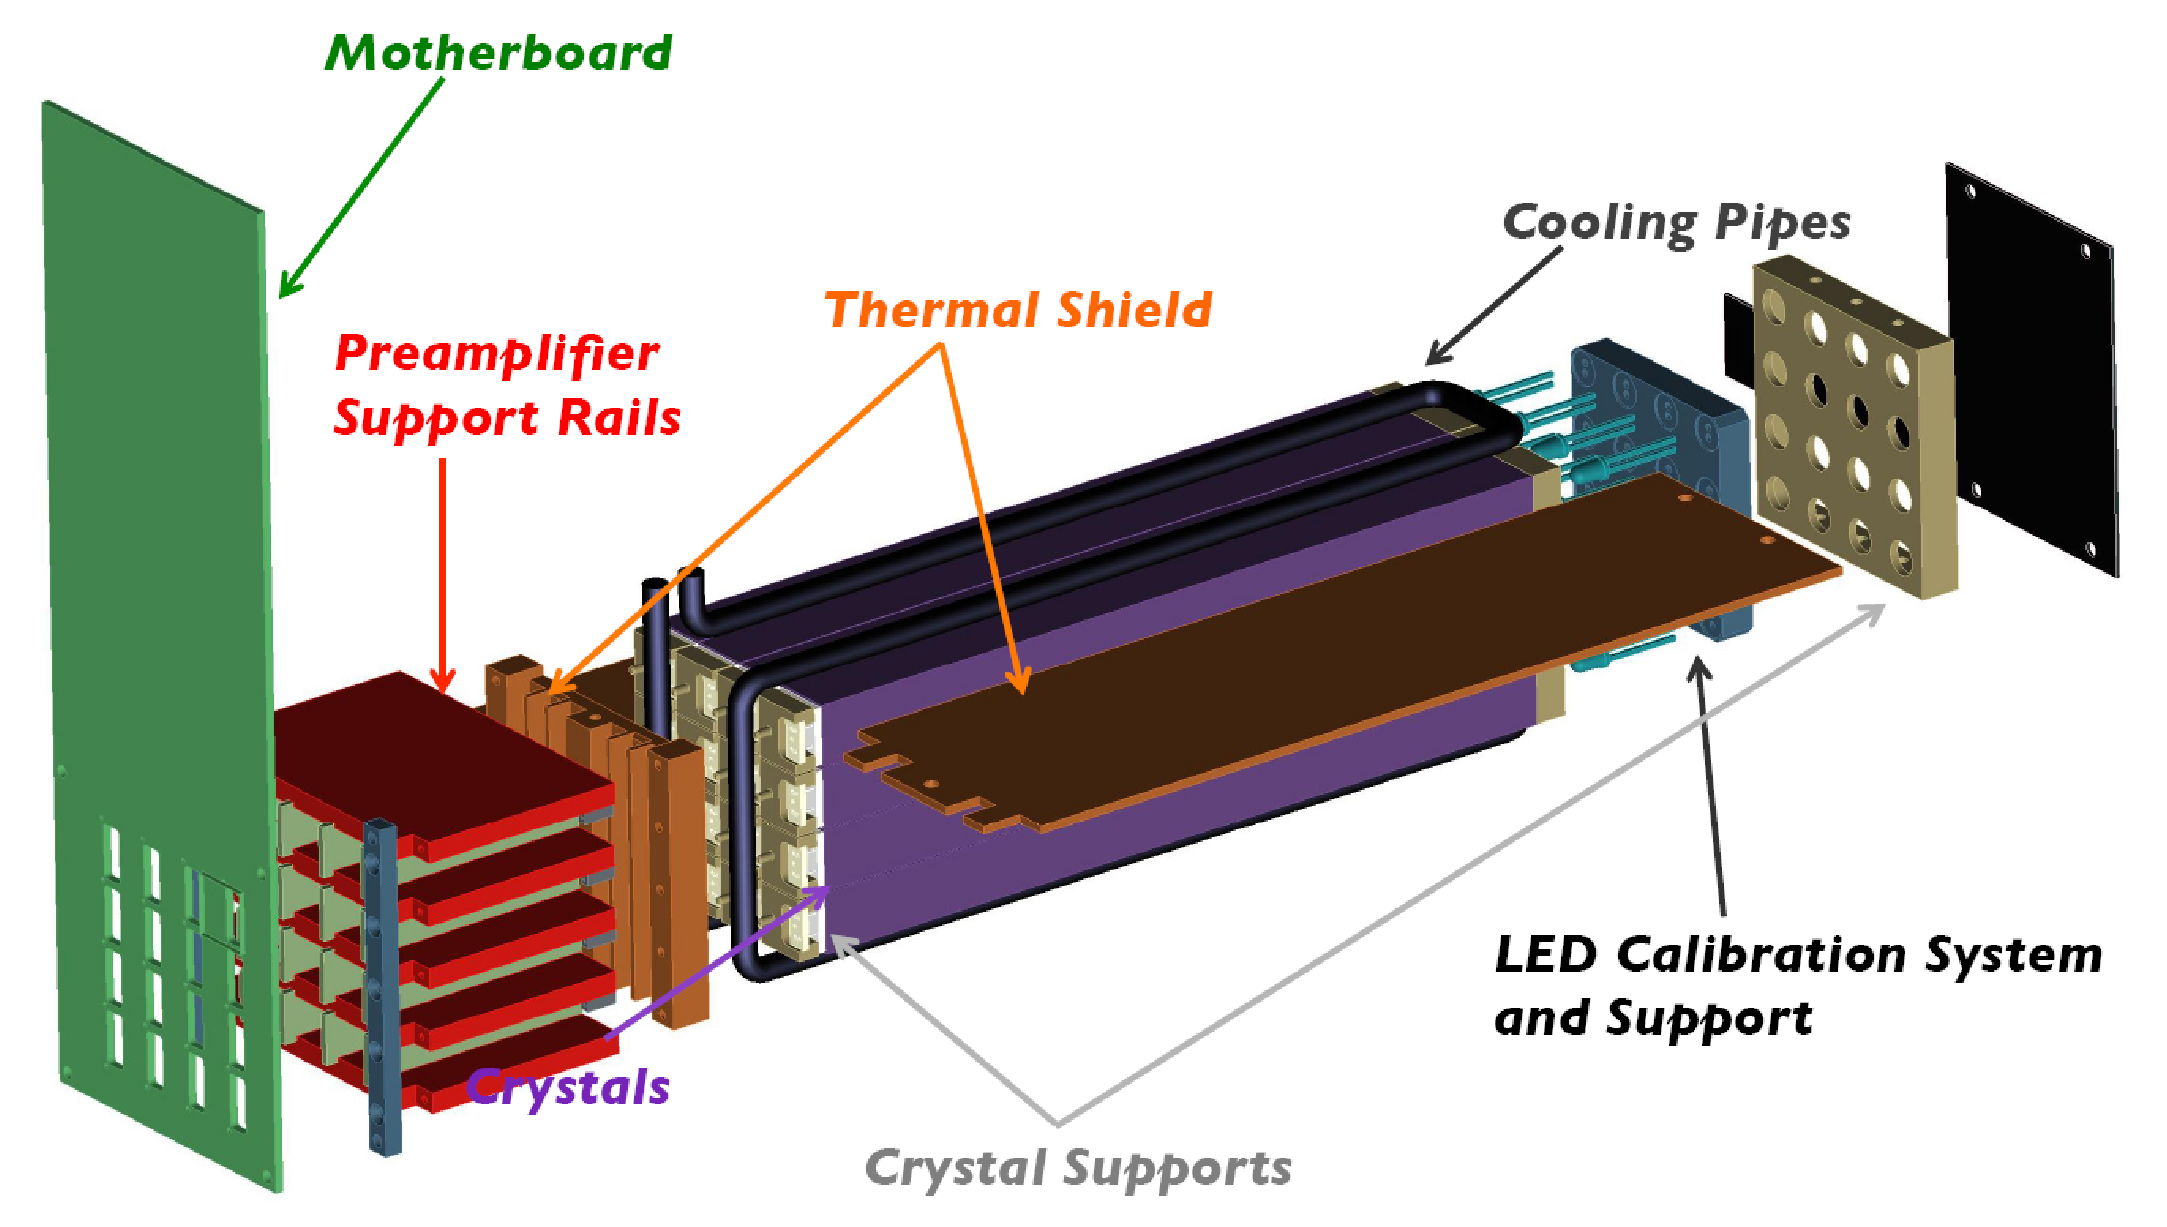
\includegraphics[width=1.0\columnwidth]{./fig/p16-whole.eps}
\caption{Exploded view of the Proto-16 assembly. From left to right, the CAD drawing shows the motherboard, the
  system of copper rails holding the preamplifiers, the copper shield back plate, the crystal assembly, the copper
  shield front plate, and the LED board.}
\label{fig:p16-whole}
\end{figure}

Figure~\ref{fig:btf} shows the BTF experimental hall after the installation of Proto-16 and the associated equipment.
The detector was placed on a movable table that could be displaced in the $x$ and $y$ direction (transverse
plane) with a 0.1-mm accuracy. This feature was exploited to center the calorimeter with respect to the beam. A
plastic scintillator bar, read out by two PMTs, was placed in front of the beam pipe exit window and was used to
determine the arrival time of the electron within the 10-ns bunch duration. The data acquisition system, based on the
JLab CODA standard~\cite{daq}, was triggered by the radio-frequency (RF) signal of the Frascati accelerator. For
each trigger all of the signals of the Proto-16 crystal matrix and of the scintillator-bar PMTs were recorded by
CAEN VME boards. Both the Proto-16 and scintillator signals were sent to a passive splitter whose two outputs were
connected the 250~MHz FADCs and to leading-edge discriminators. The discriminator output was sent to pipeline
TDCs. The samples recorded by the FADCs in an 800~ns window were recorded for each trigger and analyzed offline
to evaluate the charge and time.

\begin{figure}
\includegraphics[width=1.0\columnwidth]{./fig/btf_oct12.eps}
\caption{Experimental setup of the Proto-16 test at the LNF Beam Test Facility (BTF). Beam comes from the right.
  On the left, the detector inside its case (black) is placed on a movable table to allow for centering of the calorimeter
  with respect to the beam. In front of the calorimeter, a plastic scintillator bar wrapped in black Tedlar is used to
  determine the arrival time of the beam electrons.}
\label{fig:btf}
\end{figure}

The conversion between charge and energy was first determined using cosmic ray measurements and then optimized
by studying the response of each crystal to 500~MeV electrons at the LNF-BTF. It is worth noting that the new
calibration constants were found to be within 5-10\% of the initial values determined during cosmic-ray data
taking. The total reconstructed energy  after the full calibration is shown in Fig.~\ref{fig:btf_etot} for an electron
multiplicity of the order of 1-2. The peaks corresponding to different bunch populations are clearly visible and well
separated. 

\begin{figure}
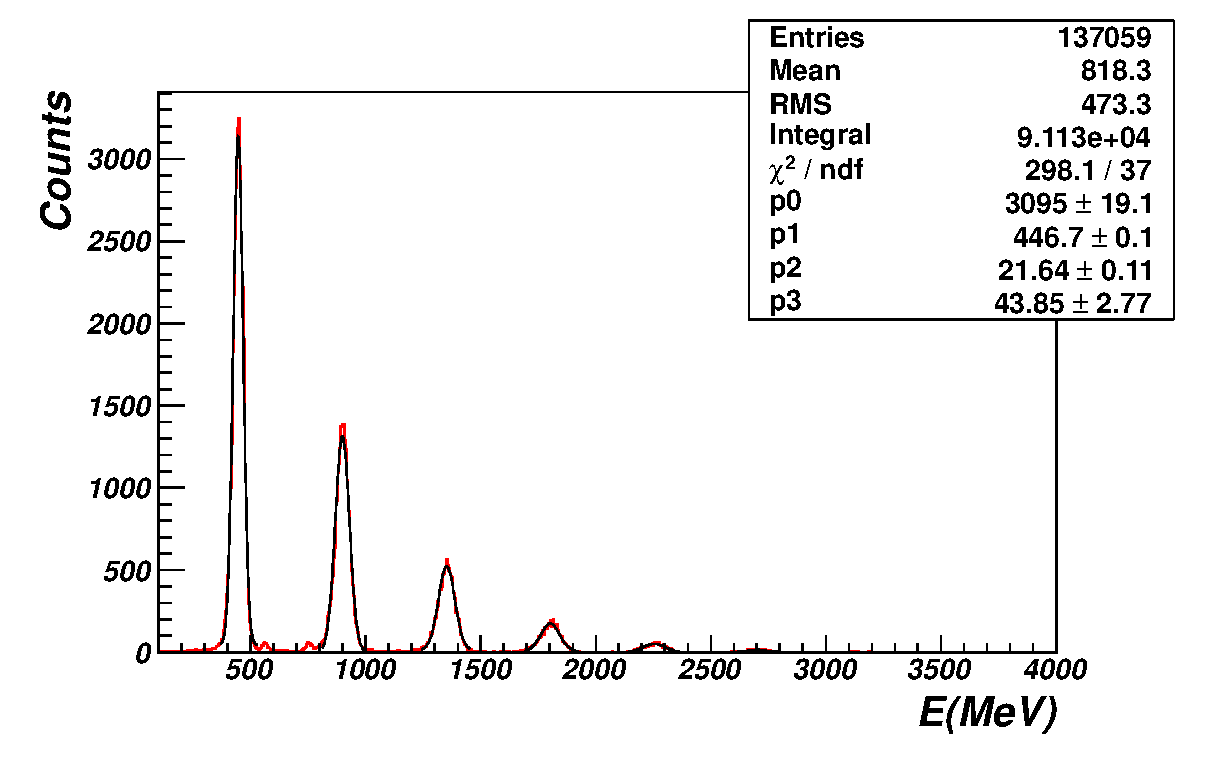
\includegraphics[width=1.0\columnwidth]{./fig/btf_etot_1876_2_6.eps}
\caption{The total energy measured by Proto-16 after calibration. The peaks correspond to different bunch
  populations and are clearly visible and well separated.}
\label{fig:btf_etot}
\end{figure}

\paragraph{Energy Resolution}

The mean values and widths ($\sigma$) of the peaks in the total reconstructed energy spectrum were analyzed to
check the system linearity and to determine the resolution. The measurements were performed by centering the
beam on the calorimeter to have the maximum containment of the electromagnetic shower.
Figure~\ref{fig:btf_linearity} shows the fitted peak position as a function of total energy in the beam bunch for an
APD gain of 150 and a PbWO$_4$ temperature of $18^{\circ}$C. The linear regression of the experimental points
shows no deviations from linearity in the explored range. The same measurement performed in different experimental
configurations gave consistent results, confirming that the system is linear up to the maximum measured energy of
4~GeV.

Figure~\ref{fig:btf_resolution} shows the energy resolution as a function of the energy in the beam bunch. The
colored points correspond to the resolution measured with Proto-16, while the black open circles are the results
of the Monte Carlo (GEMC) simulations. The error bars in the graph show the statistical uncertainty, while the
systematic uncertainty was estimated to be on the order of 5\%.  As expected, the experimental resolution
improves for increasing energy, reaching an asymptotic behavior at about 3~GeV. The measurements performed in
different configurations are in general consistent, varying within a range of 0.5\% except for the resolution obtained
at room temperature and $G$=75 (orange points). The resolution in this case is systematically worse than that
obtained at the same temperature but $G$=150. This was interpreted as due to the preamplifier noise being the
dominant factor in determining the resolution at this temperature. From this we concluded that working at higher
APD gain is the preferable configuration. 

\begin{figure}
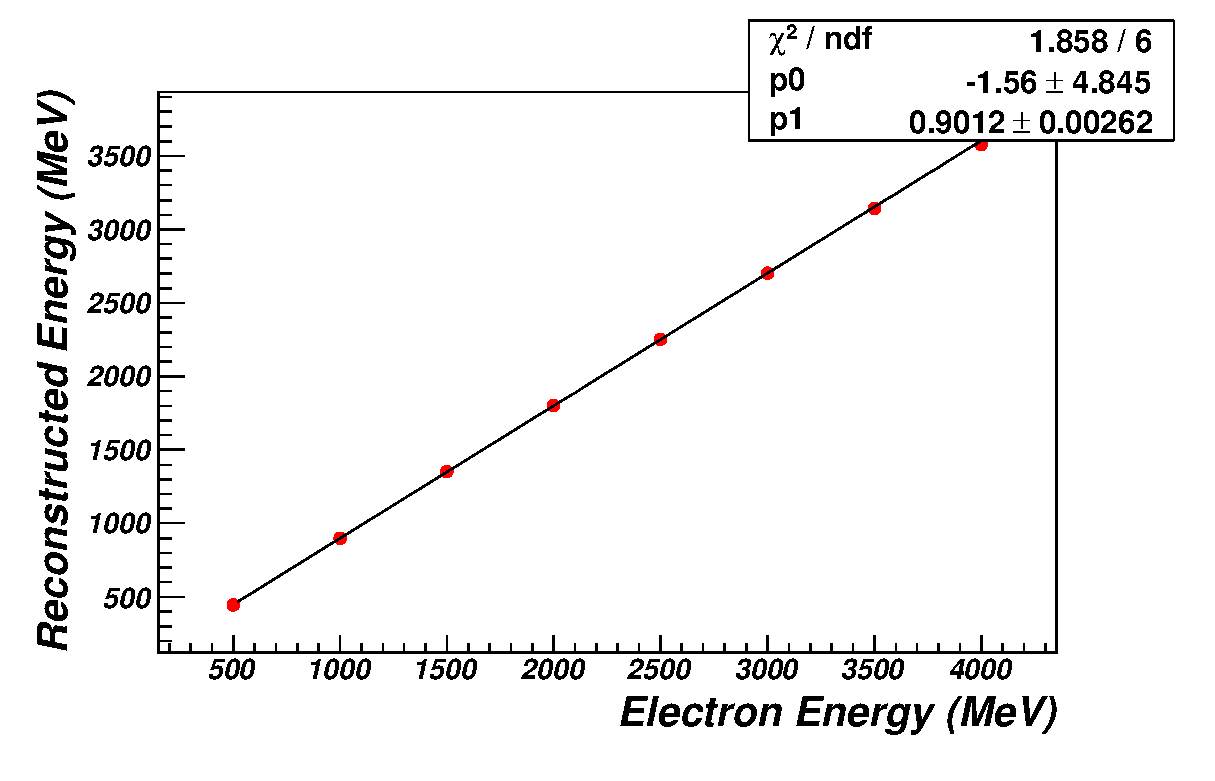
\includegraphics[width=1.0\columnwidth]{fig/btf_linearity_1876_2_6.eps}
\caption{Proto-16 reconstructed energy as a function of the beam bunch energy. The red points were obtained at
  room temperature and with an APD gain of 150. The linear regression of the experimental points shows no deviation
  from linearity.}
\label{fig:btf_linearity}
\end{figure}

The comparison of the resolution obtained at different temperatures shows that lower temperatures,
corresponding to higher light yield, and therefore larger signal, gives better resolution. The best values were
obtained at $-20^{\circ}$C, where the experimental points are in good agreement with the simulation results. The
dependence of the resolution on the temperature is more evident for high bunch energies, where threshold
effects are smaller. Above 2~GeV, the resolution at room temperature seems to be systematically higher than that
obtained at $0^\circ$C or $-20^\circ$C with a difference of about 0.5\%. The difference of the resolution obtained
at $0^\circ$C and $-20^\circ$C is on the contrary negligible within the systematic uncertainties. Based
on these results and considering the technical difficulties in operating the FT-Cal at the lowest temperature, we
concluded that the optimal operating temperature of the calorimeter is $0^\circ$C.

\begin{figure}
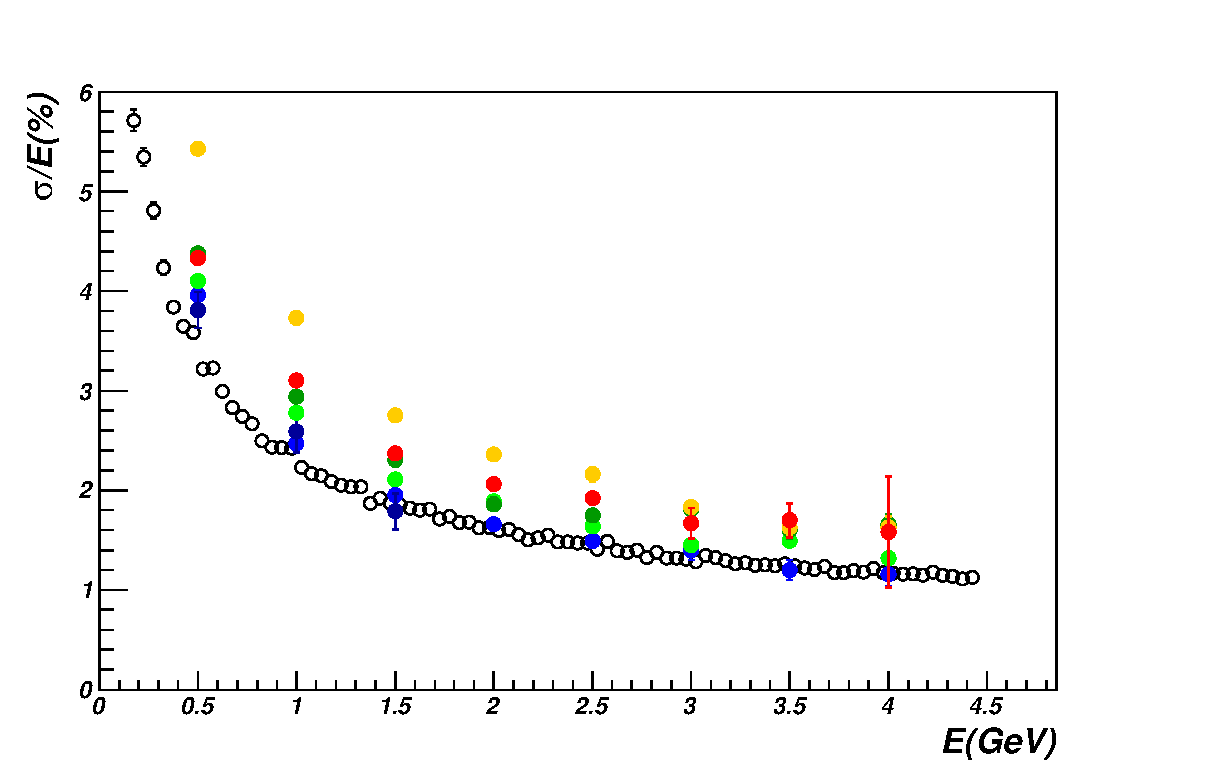
\includegraphics[width=1.0\columnwidth]{./fig/btf_resolution.eps}
\caption{Proto-16 energy resolution as a function of the beam bunch energy. The red and orange points were obtained
  at room temperature for APD gains of 150 and 75, respectively. The green points correspond to $0^\circ$C; the
  darker points were obtained removing the passive splitter. The blue and dark-blue points, that partially overlap, correspond to
  $-20^\circ$C  with APD gains of 150 and 75, respectively. The open black circles show the expected resolution based
  on Monte Carlo simulations. Only statistical uncertainties are shown.}
\label{fig:btf_resolution}
\end{figure} 
